\chapter{Grafi}

\section{Grafi non orientati}

\begin{defn}[grafo non orientato semplice]	
Un \emph{grafo non orientato semplice} $G$ è una coppia ordinata $(V,E)$ dove: $V=\{v_1,\dots,v_n\}$ è
un insieme finito di \emph{vertici} (o \emph{nodi}) ed $E$ è un insieme di coppie
\emph{non ordinate} di vertici dette \emph{spigoli}\footnote{In inglese gli spigoli sono denominati \emph{edges}, per
questo motivo l'insieme che li contiene è chiamato $E$.} o \emph{lati}. 
Il grafo è detto \emph{semplice} perché non può avere né cappi né spigoli paralleli.
\end{defn}

\begin{ese}
In Figura~\ref{fig:grf_semplice} è rappresentato il seguente grafo non orientato semplice:
\[V = \{ v_1, v_2, v_3, v_4, v_5, v_6, v_7, v_8 \}\]
\[E = \{ (v_1,v_3), (v_1,v_7), (v_2,v_3), (v_4,v_7),(v_6,v_5), (v_4,v_2), (v_3,v_5), (v_5,v_7) \}\]
Si dice che lo spigolo $(v_1,v_3)$ ha come \emph{estremi} i vertici $v_1$ e $v_3$. \QEDA
\end{ese}
\begin{figure}[H]
    \centering
    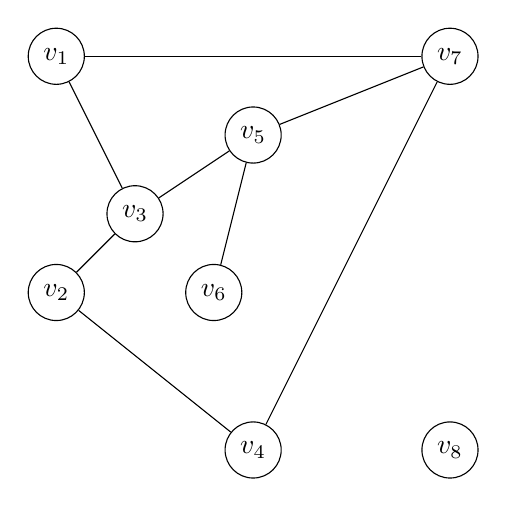
\begin{tikzpicture}
        \node[shape=circle,draw=black] (A) at (0,6) {$v_1$};
        \node[shape=circle,draw=black] (B) at (0,3) {$v_2$};
        \node[shape=circle,draw=black] (C) at (1,4) {$v_3$};
        \node[shape=circle,draw=black] (D) at (2.5,1) {$v_4$};
        \node[shape=circle,draw=black] (E) at (2.5,5) {$v_5$};
        \node[shape=circle,draw=black] (F) at (2,3) {$v_6$};
        \node[shape=circle,draw=black] (G) at (5,6) {$v_7$};
        \node[shape=circle,draw=black] (H) at (5,1) {$v_8$};

        %\path [->] (A) edge node[left] {$5$} (B);
        \path (A) edge (C);
        \path (A) edge (G);
        \path (B) edge (C);
        \path (D) edge (G);
        \path (F) edge (E);
        \path (D) edge (B);
        \path (C) edge (E);
        \path (E) edge (G);
    \end{tikzpicture}
    \caption{un grafo semplice non orientato}
    \label{fig:grf_semplice}
\end{figure}
In molti libri di testo 
$E$ viene rappresentato come ${E = \{ \text{ } \{v_i,v_j\}, \text{ } \dots, \{v_k,v_m\} \text{ } \}}$ perché non c'è
alcun ordine tra gli spigoli.
\begin{ese}
    \begin{figure}[H]
        \centering
        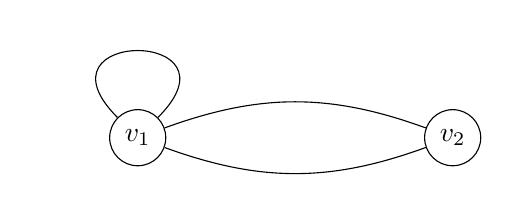
\begin{tikzpicture}[every loop/.style={}]
            \node[shape=circle,draw=black] (A) at (0,0) {$v_1$};
            \node[shape=circle,draw=black] (B) at (4,0) {$v_2$};

            \path (A) edge [loop] node {} (A);
            \path (A) edge [bend right=20] (B);
            \path (B) edge [bend right=20] (A);
        \end{tikzpicture}
        \caption{un grafo non orientato che non è semplice} \label{fig:no_semplice}
    \end{figure}
Il grafo non orientato in Figura~\ref{fig:no_semplice} non è semplice poiché presenta un
cappio sul vertice $v_1$ e ci sono due spigoli paralleli tra i vertici $v_1$ e $v_2$.
\QEDA
\end{ese}

\begin{defn}
Uno spigolo è detto \emph{incidente} nei suoi estremi. I vertici di uno spigolo sono detti \emph{adiacenti}.
\end{defn}

\begin{defn}[percorso]
	Un \emph{percorso} è una sequenza di vertici \emph{non necessariamente distinti} in cui ogni coppia di vertici consecutivi forma uno spigolo.
\end{defn}

\begin{defn}[cammino]
Un \emph{cammino} è una sequenza di vertici \emph{distinti} in cui ogni coppia di vertici consecutivi
forma uno spigolo. Alternativamente si può dire che un cammino è un percorso i cui vertici sono tutti distinti.
\end{defn}

\begin{ese}
Nel grafo in Figura~\ref{fig:camm_semplice} è presente il cammino 
${v_4 \text{ - } v_7 \text{ - } v_5 \text{ - } v_3 \text{ - } v_2 }$. Un'altra notazione
per indicare il cammino è: ${(v_4, v_7, v_5, v_3, v_2)}$. Lo stesso tipo di notazione è valido
anche per i percorsi.
    \begin{figure}[H]
        \centering
        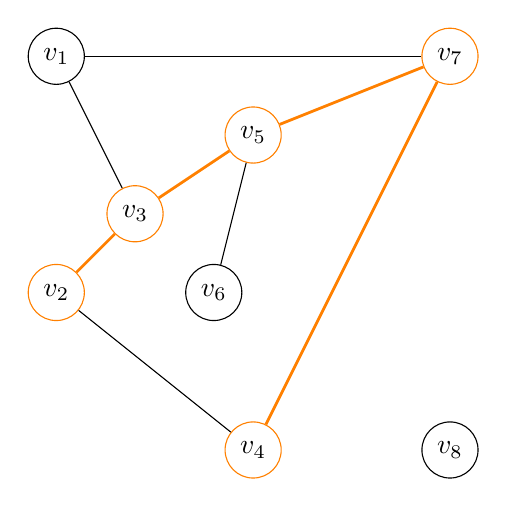
\begin{tikzpicture}
            \node[shape=circle,draw=black] (A) at (0,6) {$v_1$};
            \node[shape=circle,draw=orange] (B) at (0,3) {$v_2$};
            \node[shape=circle,draw=orange] (C) at (1,4) {$v_3$};
            \node[shape=circle,draw=orange] (D) at (2.5,1) {$v_4$};
            \node[shape=circle,draw=orange] (E) at (2.5,5) {$v_5$};
            \node[shape=circle,draw=black] (F) at (2,3) {$v_6$};
            \node[shape=circle,draw=orange] (G) at (5,6) {$v_7$};
            \node[shape=circle,draw=black] (H) at (5,1) {$v_8$};

            %\path [->] (A) edge node[left] {$5$} (B);
            \path (A) edge (C);
            \path (A) edge (G);
            \path[draw=orange,line width=0.1em] (B) edge (C);
            \path[draw=orange,line width=0.1em] (D) edge (G);
            \path (F) edge (E);
            \path (D) edge (B);
            \path[draw=orange,line width=0.1em] (C) edge (E);
            \path[draw=orange,line width=0.1em] (E) edge (G);
        \end{tikzpicture}
        \caption{un cammino $v_4 \text{ - } v_7 \text{ - } v_5 \text{ - } v_3 \text{ - } v_2 $}
        \label{fig:camm_semplice}
    \end{figure}
	\QEDA
\end{ese}

\begin{thm}
	Se un grafo contiene un percorso che ha come estremità i vertici $v_1$ e $v_n$ allora dal percorso è possibile estrarre un cammino che ha come estremità $v_1$ e $v_n$.
	\proof
	Sia $P$ un percorso che ha come estremità i vertici $v_1$ e $v_n$. Se un vertice $v_i$ (con $i \in \{1,\dots,n\}$) si ripetesse nel percorso, allora esisterebbe un sottopercorso $v_i - v_{k_1} - \dots - v_{k_h} - v_i$ contenuto in $P$. Togliendo il sottopercorso $v_i - v_{k_1} - \dots - v_{k_h}$ da $P$ si potrebbe costruire un percorso più corto. Una volta tolti da $P$ tutti i sottopercorsi che contengono nodi ripetuti, $P$ è un cammino di estremità $v_1$ e $v_n$.
	\endproof
\end{thm}

\begin{defn}[circuito]
Cammino nel quale il primo e l'ultimo vertice sono adiacenti.
\end{defn}
\begin{ese}
Il grafo in Figura~\ref{fig:circ_semplice} contiene il circuito:
$v_4 \text{ - } v_7 \text{ - } v_5 \text{ - } v_3 \text{ - } v_2 \text{ - } v_4$.
    \begin{figure}[H]
    \centering
        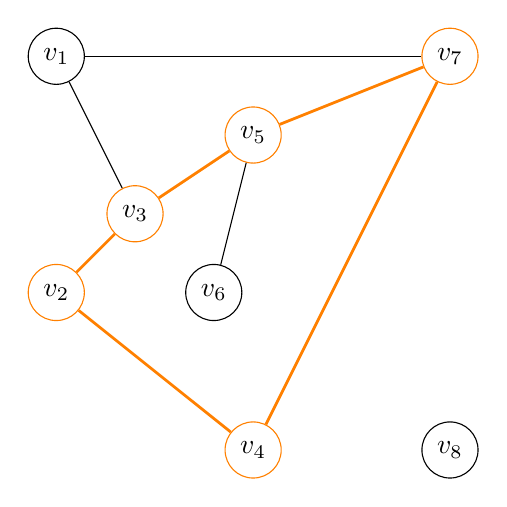
\begin{tikzpicture}
            \node[shape=circle,draw=black]  (A) at (0,6) {$v_1$};
            \node[shape=circle,draw=orange] (B) at (0,3) {$v_2$};
            \node[shape=circle,draw=orange] (C) at (1,4) {$v_3$};
            \node[shape=circle,draw=orange] (D) at (2.5,1) {$v_4$};
            \node[shape=circle,draw=orange] (E) at (2.5,5) {$v_5$};
            \node[shape=circle,draw=black]  (F) at (2,3) {$v_6$};
            \node[shape=circle,draw=orange] (G) at (5,6) {$v_7$};
            \node[shape=circle,draw=black]  (H) at (5,1) {$v_8$};

            %\path [->] (A) edge node[left] {$5$} (B);
            \path (A) edge (C);
            \path (A) edge (G);
            \path[draw=orange,line width=0.1em] (B) edge (C);
            \path[draw=orange,line width=0.1em] (D) edge (G);
            \path (F) edge (E);
            \path[draw=orange,line width=0.1em] (D) edge (B);
            \path[draw=orange,line width=0.1em] (C) edge (E);
            \path[draw=orange,line width=0.1em] (E) edge (G);
        \end{tikzpicture}
        \caption{ un circuito 
            $v_4 \text{ - } v_7 \text{ - } v_5 \text{ - } v_3 \text{ - } v_2 \text{ - } v_4$}
        \label{fig:circ_semplice}
    \end{figure}
	\QEDA
\end{ese}

\begin{defn}[lunghezza di un circuito/cammino]
La lunghezza di un circuito o di un cammino è il numero degli spigoli formati dai
nodi del cammino/circuito.
\end{defn}

%\begin{thm}
%	Un percorso chiuso di lunghezza dispari contiene un ciclo di lunghezza dispari.
%	\proof
%	\textcolor{red}{DA FARE. Per ora solamente copiato ed incollato stronzate da slides conforti}\\
%	Se gli unici vertici coincidenti sono le estremita' allora il percorso e' un ciclo dispari. Altrimenti il percorso si
%	partiziona in due percorsi di lunghezza minore, uno pari e l'altro dispari
%	\endproof
%\end{thm}

\begin{defn}[grafo connesso]
Un grafo si dice \emph{connesso} se per ogni coppia di vertici esiste un cammino
che li collega, altrimenti si dice \emph{disconnesso} o \emph{sconnesso}.
\end{defn}

\begin{defn}[grafo completo]
Un grafo è \emph{completo} se ogni sua coppia di vertici è collegata da uno spigolo.
Se un grafo completo ha $n$ vertici allora si dice che è un grafo~$k_n$.
\end{defn}
\begin{ese}
    In Figura~\ref{fig:completi} sono rappresentati 3 grafi completi.\marginnote{
        Nell'ordine:
        \begin{itemize}
            \item un grafo $k_3$
            \item un grafo $k_4$
            \item un grafo $k_5$
        \end{itemize}
    }[1cm]
    \begin{figure}[H]
    \centering
        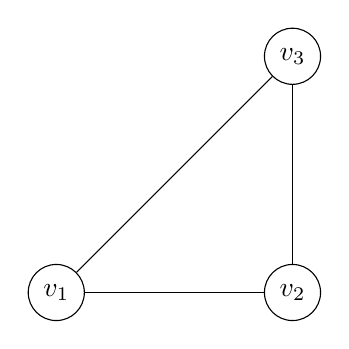
\begin{tikzpicture}
            \node[shape=circle,draw=black] (A) at (0,0) {$v_1$};
            \node[shape=circle,draw=black] (B) at (3,0) {$v_2$};
            \node[shape=circle,draw=black] (C) at (3,3) {$v_3$};

            \path (A) edge node {} (B);
            \path (A) edge node {} (C);
            \path (B) edge node {} (C);
        \end{tikzpicture}
        \hspace{1cm}
        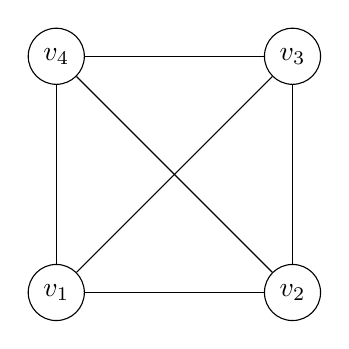
\begin{tikzpicture}
            \node[shape=circle,draw=black] (A) at (0,0) {$v_1$};
            \node[shape=circle,draw=black] (B) at (3,0) {$v_2$};
            \node[shape=circle,draw=black] (C) at (3,3) {$v_3$};
            \node[shape=circle,draw=black] (D) at (0,3) {$v_4$};

            \path (A) edge node {} (B);
            \path (A) edge node {} (C);
            \path (B) edge node {} (C);
            \path (A) edge node {} (D);
            \path (C) edge node {} (D);
            \path (B) edge node {} (D);

        \end{tikzpicture}
        \hspace{1cm}
        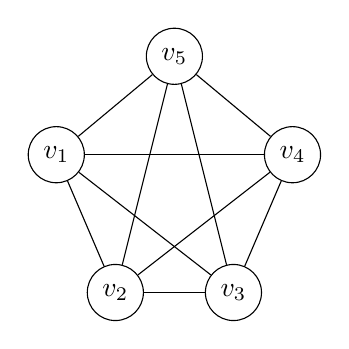
\begin{tikzpicture}
            \node[shape=circle,draw=black] (A) at (0,1.75) {$v_1$};
            \node[shape=circle,draw=black] (B) at (0.75,0) {$v_2$};
            \node[shape=circle,draw=black] (C) at (2.25,0) {$v_3$};
            \node[shape=circle,draw=black] (D) at (3,1.75) {$v_4$};
            \node[shape=circle,draw=black] (E) at (1.5,3) {$v_5$};

            \path (A) edge node {} (B);
            \path (A) edge node {} (C);
            \path (A) edge node {} (D);
            \path (A) edge node {} (E);
            \path (B) edge node {} (C);
            \path (B) edge node {} (D);
            \path (B) edge node {} (E);
            \path (C) edge node {} (D);
            \path (C) edge node {} (E);
            \path (D) edge node {} (E);
        \end{tikzpicture}
        \caption{un $k_3$, $k_4$ e $k_5$} \label{fig:completi}
    \end{figure}
	\QEDA
\end{ese}

\begin{defn}[grafo bipartito]   \label{bip}
Un grafo $G = (V,E)$ è \emph{bipartito} se i suoi vertici sono partizionati in due sottoinsiemi di $V$, 
rispettivamente $U$ e $W$, ed ogni suo spigolo è incidente in un vertice di $U$ ed in uno di $W$
(notare che ${U \cap W = \emptyset}$ e ${U \cup W = V}$).
\end{defn}

\begin{ese}
Due grafi bipartiti sono rappresentati in Figura~\ref{fig:bipartiti}.
    \begin{figure}[H]
    \centering
        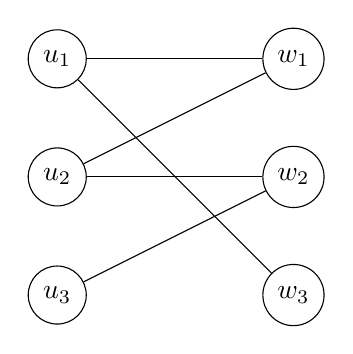
\begin{tikzpicture}
            \node[shape=circle,draw=black] (A) at (0,3) {$u_1$};
            \node[shape=circle,draw=black] (B) at (3,3) {$w_1$};
            \node[shape=circle,draw=black] (C) at (0,1.5) {$u_2$};
            \node[shape=circle,draw=black] (D) at (3,1.5) {$w_2$};
            \node[shape=circle,draw=black] (E) at (0,0) {$u_3$};
            \node[shape=circle,draw=black] (F) at (3,0) {$w_3$};

            \path (A) edge node {} (B);
            \path (A) edge node {} (F);
            \path (B) edge node {} (C);
            \path (C) edge node {} (D);
            \path (D) edge node {} (E);
        \end{tikzpicture}
        \hspace{1cm}
        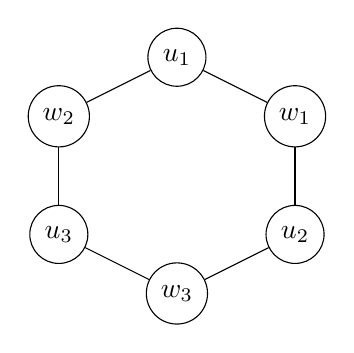
\begin{tikzpicture}
            \node[shape=circle,draw=black] (A) at (1.5, 3) {$u_1$};
            \node[shape=circle,draw=black] (B) at (3, 2.25) {$w_1$};
            \node[shape=circle,draw=black] (C) at (3, 0.75) {$u_2$};
            \node[shape=circle,draw=black] (D) at (0, 2.25) {$w_2$};
            \node[shape=circle,draw=black] (E) at (0, 0.75) {$u_3$};
            \node[shape=circle,draw=black] (F) at (1.5, 0) {$w_3$};

            \path (A) edge node {} (D);
            \path (A) edge node {} (B);
            \path (B) edge node {} (C);
            \path (F) edge node {} (E);
            \path (F) edge node {} (C);
            \path (B) edge node {} (C);
            \path (D) edge node {} (E);
        \end{tikzpicture}
        \caption{2 grafi bipartiti} \label{fig:bipartiti}
    \end{figure}
	\QEDA
\end{ese}

\begin{defn}[grafo bipartito completo $k_{n_1, n_2}$]  
	Un grafo bipartito è \emph{completo} se tutti i suoi vertici partizionati in un sottoinsieme
	sono adiacenti a tutti i vertici dell'altro sottoinsieme.
\end{defn}

\begin{ese}
	Due grafi bipartiti completi sono rappresentati in Figura~\ref{fig:bipartiti_completi}.\marginnote{
		Nell'ordine:
		\begin{itemize}
			\item un grafo $k_{1,3}$
			\item un grafo $k_{2,4}$
		\end{itemize}
	}[0.5cm]
	\begin{figure}[H]
		\centering
		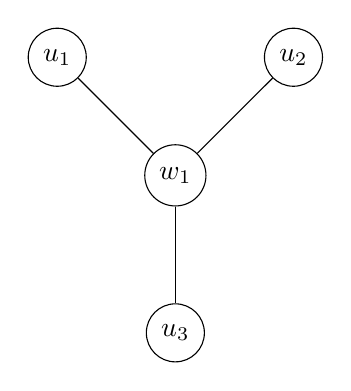
\begin{tikzpicture}
		\node[shape=circle,draw=black] (A) at (0,1.5) {$u_1$};
		\node[shape=circle,draw=black] (B) at (1.5,0) {$w_1$};
		\node[shape=circle,draw=black] (C) at (3,1.5) {$u_2$};
		\node[shape=circle,draw=black] (D) at (1.5,-2) {$u_3$};
		
		\path (A) edge node {} (B);
		\path (B) edge node {} (C);
		\path (B) edge node {} (D);
		
		\end{tikzpicture}
		\hspace{1cm}
		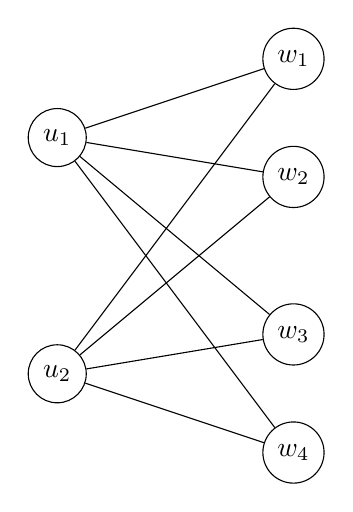
\begin{tikzpicture}
		\node[shape=circle,draw=black] (A) at (0,-1) {$u_1$};
		\node[shape=circle,draw=black] (B) at (0,-4) {$u_2$};
		\node[shape=circle,draw=black] (C) at (3,0) {$w_1$};
		\node[shape=circle,draw=black] (D) at (3,-1.5) {$w_2$};
		\node[shape=circle,draw=black] (E) at (3,-3.5) {$w_3$};
		\node[shape=circle,draw=black] (F) at (3,-5) {$w_4$};
		
		\path (A) edge node {} (C);
		\path (A) edge node {} (D);
		\path (A) edge node {} (E);
		\path (A) edge node {} (F);
		\path (B) edge node {} (C);
		\path (B) edge node {} (D);
		\path (B) edge node {} (E);
		\path (B) edge node {} (F);
		\end{tikzpicture}
		\caption{2 grafi bipartiti completi} \label{fig:bipartiti_completi}
	\end{figure}
	\QEDA
\end{ese}

\begin{defn}[foresta]
	Una \emph{foresta} è un grafo senza cicli (\emph{aciclico}).
\end{defn}
\begin{ese}
	In Figura~\ref{fig:foresta} è rappresentata una foresta.
	\begin{figure}[H]
		\centering
		\begin{tikzpicture}
		\begin{scope}[every node/.style={circle,thick,draw,
			inner sep=0pt, minimum size=9pt}]
		\node (A) at (0,0) {};
		\node (B) at (1.5,2) {};
		\node (C) at (3,0.5) {};
		\node (D) at (-2,1.5) {};
		\node (E) at (0,-1.5) {};
		\node (F) at (1.5,-1) {};
		\end{scope}
		
		\path (A) edge node {} (B);
		\path (B) edge node {} (C);
		\path (A) edge node {} (D);
		\path (A) edge node {} (E);
		\path (E) edge node {} (F);
		\end{tikzpicture}
		\caption{Una foresta} \label{fig:foresta}
	\end{figure}
	\QEDA
\end{ese}

\begin{defn}[albero]
	Un \emph{albero} è una foresta connessa.
\end{defn}

\textcolor{red}{SPOSTARE FORESTA E GRAFO (AGGIUNGENDO ESEMPIO PER QUEST'ULTIMO) DOPO AVER CREATO UN CAPITOLO SUGLI ALBERI}\\
\textcolor{green}{aggiungere una sezione per i multigrafi}

\section{Grafi orientati}
\begin{defn}[grafo orientato semplice]
Un \emph{grafo orientato semplice} $G$ è una coppia ordinata $(V, A)$ dove:
$V = \{ v_1, \dots, v_n \}$ è un insieme finito di vertici (o nodi) ed
$A$ è un insieme di \emph{coppie ordinate} di vertici dette \emph{archi}.
\end{defn}

\begin{ese}
\[G = (V,A) \text{ con } V = \{ v_1, v_2, v_3, v_4, v_5 \} \text{ e} \]
\[A = \{ (v_1, v_3), (v_2, v_1), (v_2, v_5), (v_3, v_5), (v_4, v_1), (v_4, v_3), (v_5, v_2) \} \]
    \begin{figure}[H]
    \centering
        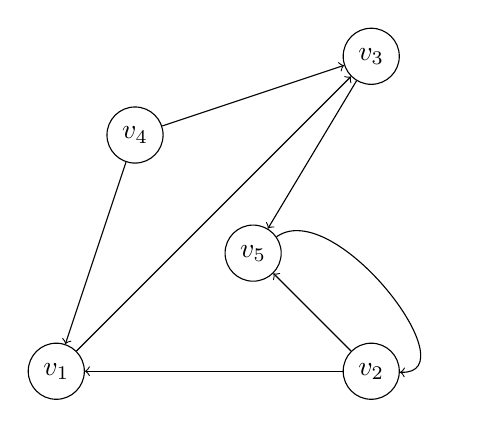
\begin{tikzpicture}
            \node[shape=circle,draw=black] (A) at (0,0) {$v_1$};
            \node[shape=circle,draw=black] (B) at (4,0) {$v_2$};
            \node[shape=circle,draw=black] (C) at (4,4) {$v_3$};
            \node[shape=circle,draw=black] (D) at (1,3) {$v_4$};
            \node[shape=circle,draw=black] (E) at (2.5,1.5) {$v_5$};

            \path [->] (A) edge node[left] {} (C);
            \path [->] (B) edge node[left] {} (A);
            \path [->] (B) edge node[left] {} (E);
            \path [->] (C) edge node[left] {} (E);
            \path [->] (D) edge node[left] {} (A);
            \path [->] (D) edge node[left] {} (C);
            \path [->] (E) edge [out=35,in=-2] node[left] {} (B);
        \end{tikzpicture}
        \caption{un grafo orientato semplice}
        \label{fig:grf_or_semplice}
    \end{figure}
	\QEDA
\end{ese}
Il grafo è semplice perché non ha né cappi né archi paralleli. %Essendo orientato
%il grafo ha un \emph{nodo iniziale} (\emph{testa}) ed un \emph{nodo finale} (\emph{coda}).
Il nodo iniziale di un arco è detto \emph{testa} e quello finale è detto \emph{coda}.

\begin{ese}
\[ G=(V, A) \quad V = \{v_1, v_2\} \quad A = \{ (v_1, v_2), (v_2, v_1) \}\]
$G$ è un grafo orientato. L'arco $(v_1, v_2) \in A$ ha $v_1$ come nodo iniziale
e $v_2$ come finale.
    \begin{figure}[H]
    \centering
        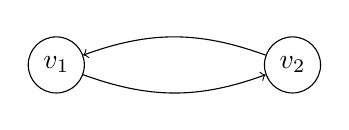
\begin{tikzpicture}
            \node[shape=circle,draw=black] (A) at (0, 0) {$v_1$};
            \node[shape=circle,draw=black] (B) at (3, 0) {$v_2$};

            \path [->] (A) edge [bend right=20] node[right] {} (B);
            \path [->] (B) edge [bend right=20] node[left] {} (A);
        \end{tikzpicture}
        \caption{un grafo orientato semplice}
        \label{fig:grf_or_non_semplice}
    \end{figure}
\QEDA
\end{ese}

\begin{ese}
L'immagine in Figura~\ref{fig:no_orientato_semplice} non rappresenta un grafo orientato semplice
perché i vertici $v_1$ e $v_2$ sono collegati da due archi paralleli 
(ovvero due archi che hanno lo stesso nodo iniziale ed anche quello finale), 
inoltre c'è un cappio su $v_1$.
    \begin{figure}[H] 
    \centering
        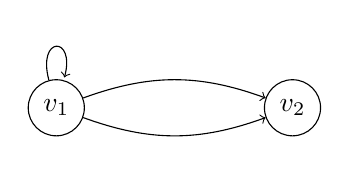
\begin{tikzpicture}
            \node[shape=circle,draw=black] (A) at (0, 0) {$v_1$};
            \node[shape=circle,draw=black] (B) at (3, 0) {$v_2$};

            \path (A) edge [loop above] node {} (A);
            \path [->] (A) edge [bend right=20] node[right] {} (B);
            \path [->] (A) edge [bend left=20] node[right] {} (B);
        \end{tikzpicture}
        \caption{grafo orientato che non è semplice (un \emph{multigrafo} orientato)}
        \label{fig:no_orientato_semplice}
    \end{figure}
\QEDA
\end{ese}

\begin{defn}[cammino orientato]
Un \emph{cammino orientato} è una sequenza di nodi distinti dove, ogni coppia di nodi
consecutivi nel cammino è collegata da un arco.
\end{defn}

\begin{ese}
Nel grafo in Figura~\ref{fig:cammino_orientato} è presente il cammino orientato: 
\[v_1 - v_3 - v_5 - v_2\]
    \begin{figure}[H]
    \centering
        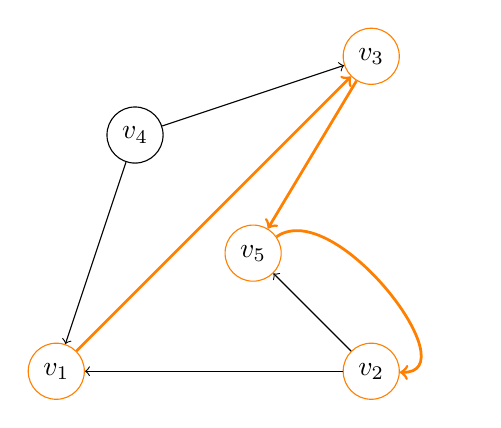
\begin{tikzpicture}
            \node[shape=circle,draw=orange] (A) at (0,0) {$v_1$};
            \node[shape=circle,draw=orange] (B) at (4,0) {$v_2$};
            \node[shape=circle,draw=orange] (C) at (4,4) {$v_3$};
            \node[shape=circle,draw=black] (D) at (1,3) {$v_4$};
            \node[shape=circle,draw=orange] (E) at (2.5,1.5) {$v_5$};

            \path [->] (B) edge node[left] {} (A);
            \path [draw=orange,line width=0.1em][->] (A) edge node[left] {} (C);
            \path [->] (B) edge node[left] {} (E);
            \path [draw=orange,line width=0.1em][->] (C) edge node[left] {} (E);
            \path [->] (D) edge node[left] {} (A);
            \path [->] (D) edge node[left] {} (C);
            \path [draw=orange,line width=0.1em][->] (E) edge [out=35,in=-2] node[left] {} (B);
        \end{tikzpicture}
        \caption{cammino orientato} \label{fig:cammino_orientato}
    \end{figure}
\QEDA
\end{ese}

\begin{defn}[circuito orientato]
Cammino orientato nel quale esiste un arco dal primo all'ultimo nodo.
\end{defn}

\begin{ese}
In Figura~\ref{fig:c_or} è rappresentato il circuito orientato \[v_1 - v_3 - v_5 - v_2 - v_1\]
    \begin{figure}[H]
    \centering
        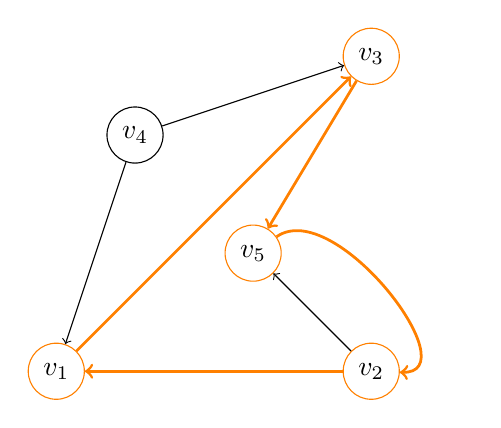
\begin{tikzpicture}
            \node[shape=circle,draw=orange] (A) at (0,0) {$v_1$};
            \node[shape=circle,draw=orange] (B) at (4,0) {$v_2$};
            \node[shape=circle,draw=orange] (C) at (4,4) {$v_3$};
            \node[shape=circle,draw=black] (D) at (1,3) {$v_4$};
            \node[shape=circle,draw=orange] (E) at (2.5,1.5) {$v_5$};

            \path [draw=orange,line width=0.1em][->] (B) edge node[left] {} (A);
            \path [draw=orange,line width=0.1em][->] (A) edge node[left] {} (C);
            \path [->] (B) edge node[left] {} (E);
            \path [draw=orange,line width=0.1em][->] (C) edge node[left] {} (E);
            \path [->] (D) edge node[left] {} (A);
            \path [->] (D) edge node[left] {} (C);
            \path [draw=orange,line width=0.1em][->] (E) edge [out=35,in=-2] node[left] {} (B);
        \end{tikzpicture}
        \caption{circuito orientato} \label{fig:c_or}
    \end{figure}
\QEDA
\end{ese}

\begin{defn}[grafo fortemente connesso]
Per ogni coppia di nodi esiste un cammino orientato che li collega. 
\end{defn}

\begin{ese}
	\[ G( V = \{ v_1, v_2, v_3 \}, \
    A = \{ (v_2, v_1), (v_1, v_3), (v_3, v_1),  (v_3, v_2) \}) \]
    è un grafo fortemente connesso ed è in Figura~\ref{fig:forte_connesso}
    \begin{figure}[H]
        \centering
            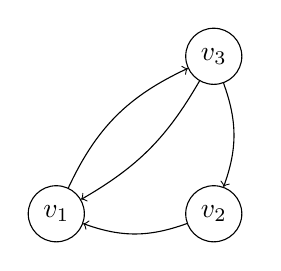
\begin{tikzpicture}
                \node[shape=circle,draw=black] (A) at (0,0) {$v_1$};
                \node[shape=circle,draw=black] (B) at (2,0) {$v_2$};
                \node[shape=circle,draw=black] (C) at (2,2) {$v_3$};

                %\path [->] (A) edge [bend left=20] node[right] {} (B);
                \path [->] (B) edge [bend left=20] node[right] {} (A);
                \path [->] (A) edge [bend left=20] node[right] {} (C);
                \path [->] (C) edge [bend left=15] node[right] {} (A);
                %\path [->] (B) edge [bend right=20] node[right] {} (C);
                \path [->] (C) edge [bend left=20] node[right] {} (B);%right=20] node[right] {} (B);
            \end{tikzpicture}
            \caption{grafo fortemente connesso} \label{fig:forte_connesso}
    \end{figure}
\QEDA
\end{ese}

\begin{defn}[torneo]
	Un torneo è un grafo orientato semplice in cui ogni coppia di vertici \emph{distinti} è 
	collegata da un arco (che può avere qualsiasi direzione ovvero, dati $u,v \in V$  può essere $(u,v)$ oppure $(v,u)$). È chiamato torneo perché, un tale grafo di $n$ nodi corrisponde a un torneo in cui ogni membro di un gruppo di $n$ giocatori gioca contro tutti gli altri $n-1$ giocatori e ad ogni partita un giocatore vince e l'altro perde.
\end{defn}
\begin{ese}
	In Figura~\ref{fig:torneo} è rappresentato un torneo.
	\begin{figure}[H]
		\centering
		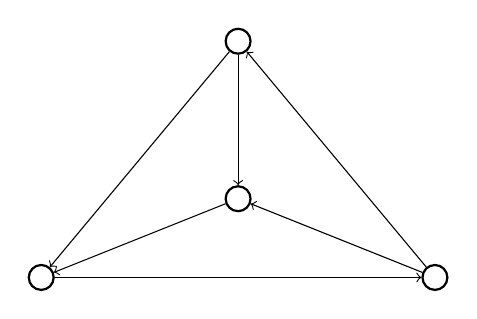
\begin{tikzpicture}
		\begin{scope}[every node/.style={circle,thick,draw,%fill=black,
				inner sep=0pt, minimum size=9pt}]
			\node (A) at (0,0) {};
			\node (B) at (-2.5,-3) {};
			\node (C) at (2.5,-3) {};
			\node (D) at (0,-2) {};
		\end{scope}
		
		\path [->] (A) edge node {} (B);
		\path [->] (C) edge node {} (A);
		\path [->] (A) edge node {} (D);
		\path [->] (B) edge node {} (C);
		\path [->] (D) edge node {} (B);
		\path [->] (C) edge node {} (D);
		\end{tikzpicture}
		\caption{Un torneo} \label{fig:torneo}
	\end{figure}
\QEDA
\end{ese}

\section{Prime proprietà dei grafi non orientati}

Sia $G=(V,E)$ un grafo non orientato semplice.
Non è difficile notare che il minimo numero di spigoli che un grafo può avere è $0$ (ogni vertice è isolato) mentre il massimo è:
\[ \frac{|V|\text{ }(|V|-1)}{2} \]
($|V|$ indica la \emph{cardinalità} di $V$. La cardinalità di un insieme finito è un numero naturale che rappresenta la quantità di elementi che costituiscono l'insieme.)
\begin{ese} In Figura~\ref{fig:card} sono rappresentati dei grafi che hanno il massimo
numero di spigoli che è possibile avere rispetto al numero dei loro vertici $|V| = 3$ e $|V| = 4$.
\begin{figure}[H]		
    \centering
        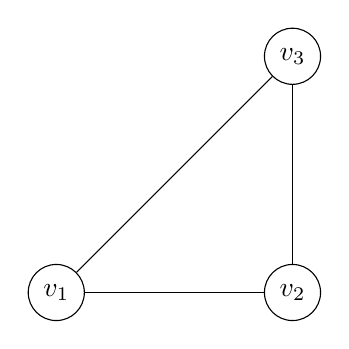
\begin{tikzpicture}
            \node[shape=circle,draw=black] (A) at (0,0) {$v_1$};
            \node[shape=circle,draw=black] (B) at (3,0) {$v_2$};
            \node[shape=circle,draw=black] (C) at (3,3) {$v_3$};

            \path (A) edge node {} (B);
            \path (A) edge node {} (C);
            \path (B) edge node {} (C);
        \end{tikzpicture}
        \hspace{1cm}
        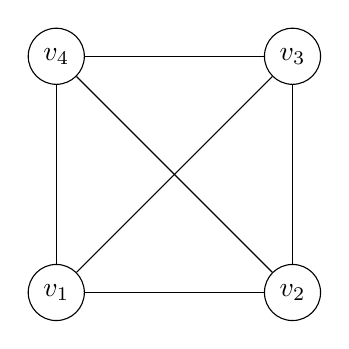
\begin{tikzpicture}
            \node[shape=circle,draw=black] (A) at (0,0) {$v_1$};
            \node[shape=circle,draw=black] (B) at (3,0) {$v_2$};
            \node[shape=circle,draw=black] (C) at (3,3) {$v_3$};
            \node[shape=circle,draw=black] (D) at (0,3) {$v_4$};

            \path (A) edge node {} (B);
            \path (A) edge node {} (C);
            \path (B) edge node {} (C);
            \path (A) edge node {} (D);
            \path (C) edge node {} (D);
            \path (B) edge node {} (D);

        \end{tikzpicture}
        \caption{due grafi rispettivamente con $|V| = 3$ e $|V| = 4$} \label{fig:card}
    \end{figure}
\QEDA
\end{ese}

\begin{defn}[grado di un vertice] Si chiama \emph{grado} di un vertice $v$ e si indica con $gr(v)$ il
numero di spigoli incidenti in $v$.
\end{defn}

\begin{ese}
	$gr(v_1) = 1$, \quad $gr(v_2) = 3$, \quad $gr(v_3) = gr(v_4) = gr(v_5) = 2$.
	\[\sum_{v \in V}^{} gr(v) = 1 + 3 + 2 + 2 + 2 = 10 = 2 |E| = 2 \times 5\]
    Il grafo relativo all'esempio è in~\ref{fig:esempio_grado}

	\begin{figure}[H]
	  	 \centering
	        \begin{tikzpicture}
		        \node[shape=circle,draw=black] (A) at (0,0) {$v_4$};
		        \node[shape=circle,draw=black] (B) at (3,0) {$v_5$};
		        \node[shape=circle,draw=black] (C) at (3,3) {$v_2$};
		        \node[shape=circle,draw=black] (D) at (0,3) {$v_3$};
		        \node[shape=circle,draw=black] (E) at (6,3) {$v_1$};

		        \path (C) edge node {} (E);
				\path (A) edge node {} (B);
		        \path (B) edge node {} (C);
		        \path (A) edge node {} (D);
		        \path (C) edge node {} (D);

	    	\end{tikzpicture}
            \caption{} \label{fig:esempio_grado}
	\end{figure}
\QEDA
\end{ese}

\begin{thm}
In ogni grafo semplice non orientato $G=(V,E)$, la somma dei gradi di tutti i vertici è
uguale al doppio del numero degli spigoli.
\begin{equation} \label{eq:thm1} \sum_{v \in V}^{} gr(v) = 2|E| \end{equation}
\proof
	Per induzione su $m = |E|$:\\
	\emph{caso base: $m = 0$}\\	
	\indent $gr(v) = 0 \quad \forall v \in V$, \quad $|E| = 0$.\\
	\emph{passo induttivo:} $P(m-1) \implies P(m)$\\
	\indent sia $G=(V,E)$ un grafo con $m$ spigoli. Si suppone che ~\ref{eq:thm1} 
	sia valida $\forall$ grafo con $m-1$ spigoli.\\
	Siano $(\bar{u}, \bar{v}) \in E$ e $G'=(V, E'=E \setminus \{(\bar{u}, \bar{v})\})$ ottenuto da $G$ togliendo 
	$(\bar{u}, \bar{v})$.\\
	Si può notare che $gr_G(\bar{u})= gr_{G'}(\bar{u})+1$, $gr_G(\bar{v}) = gr_{G'}(\bar{v})+1$ mentre,
	$\forall x \in V$ tale che $x \neq \bar{u}, x \neq \bar{v}$ si ha $ gr_G(x) = gr_{G'}(x)$.\\%https://tex.stackexchange.com/questions/10850/stop-latex-from-breaking-an-inline-math-equation
	$|E'| = |E|-1 = m -1 \implies$ in $G'$ vale l'ipotesi induttiva 
    ${\implies \sum_{v \in V}^{} gr_{G'}(v) = 2|E'|}$.\\In $G$:
    \begin{equation*}%https://it.sharelatex.com/learn/Aligning_equations_with_amsmath
    \begin{split}
	 \sum_{v \in V}^{} gr(v) & = 
     \sum_{\substack{v \in V \\ v \neq \bar{u} \\ v \neq \bar{v}} }^{} 
        gr_G=(v)+gr_G(\bar{u})+gr_G(\bar{v}) \\ & =
	 \sum_{\substack{v\in V \\ v\neq \bar{u} \\ v\neq \bar{v}} }^{} 
        gr_{G'}(v)+gr_{G'}(\bar{u})+1 +gr_{G'}(\bar{v}) +1 \\ & =
	 \sum_{v \in V}^{} gr_{G'}(v) + 2 \underbrace{=}_{\text{ipotesi induttiva}} 2|E'| + 2 \\
     & = 2(m-1) + 2 \\
	 & = 2m \\ & = 2|E|
    \end{split}
    \end{equation*}
\endproof
\end{thm}

\begin{cor}
    In ogni grafo non orientato, il numero dei vertici di grado dispari è pari.
\proof
    Siano $G=(V,E)$ un grafo non orientato semplice, ${V_d = \{v \in V \mid gr(v) \text{ è dispari}\}}$ e
    ${V_p = \{v \in V \mid gr(v) \text{ è pari}\}}$; quindi ${V_d \cap V_p = \emptyset}$ e 
    ${V_d \cup V_p = V}$.
    \begin{equation*}
    \begin{split}
        \sum_{v \in V}^{} gr(v) & = 
        2|E| \\ & = 
        \underbrace{{\sum_{v \in V_p}^{} gr(v)}}_{\text{pari}} + {\sum_{v \in V_d}^{} gr(v)} = 
        \underbrace{2|E|}_{\text{pari}}
    \end{split}
    \end{equation*}
    Poichè la somma dei gradi dei vertici che hanno grado pari è un numero pari, 
    allora anche la somma dei gradi dei vertici che hanno grado dispari è un numero pari perché:
    \[
        {\sum_{v \in V_d}^{} gr(v)} = \underbrace{2|E|}_{\text{pari}} - 
                \underbrace{{\sum_{v \in V_p}^{} gr(v)}}_{\text{pari}}
    \]
    e la differenza tra due numeri pari è un numero pari. Essendo quindi la somma dei gradi dei vertici
    di grado dispari un numero pari, allora anche il numero dei vertici di grado dispari è un numero
    pari. Questo perchè se si sommano $n$ numeri dispari, la loro somma è un numero pari 
    se e solo se $n$ è pari.
\endproof
\end{cor}

\begin{eser}
    Trovare $G=(V,E)$ con $|V| = 7$ e ${gr(v) = 5 \text{ } \forall v \in V}$.\\
    Svolgimento: non esiste alcun grafo di questo tipo, per il corollario di cui sopra.
    Infatti ho $7$ vertici di grado dispari ma, il numero dei vertici di grado dispari
    deve essere un numero pari, assurdo. \QEDA
\end{eser}




\section{Prime proprietà dei grafi orientati}
Sia $G=(V,A)$ un grafo orientato semplice. Allora il minimo numero di archi che questo può
avere è $0$ (ogni vertice è isolato) mentre il massimo è ${|V| \cdot (|V|-1)}$.

\begin{ese}
Due grafi orientati con il loro massimo numero di archi possibili sono rappresentati in 
Figura~\ref{fig:in_out_deg}
    \begin{figure}[h]
    \centering
        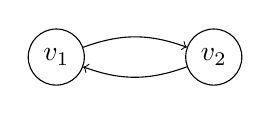
\begin{tikzpicture}
            \node[shape=circle,draw=black] (A) at (0,0) {$v_1$};
            \node[shape=circle,draw=black] (B) at (2,0) {$v_2$};

            \path [->] (A) edge [bend left=20] node[right] {} (B);
            \path [->] (B) edge [bend left=20] node[right] {} (A);
        \end{tikzpicture}
        \hspace{1cm}
        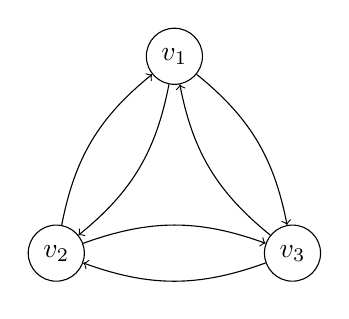
\begin{tikzpicture}
            \node[shape=circle,draw=black] (A) at (0,0) {$v_1$};
            \node[shape=circle,draw=black] (B) at (-1.5, -2.5) {$v_2$};
            \node[shape=circle,draw=black] (C) at (1.5, -2.5) {$v_3$};

            \path [->] (A) edge [bend left=20] node[right] {} (B);
            \path [->] (A) edge [bend left=20] node[right] {} (C);
            \path [->] (B) edge [bend left=20] node[right] {} (C);
            \path [->] (B) edge [bend left=20] node[right] {} (A);
            \path [->] (C) edge [bend left=20] node[right] {} (B);
            \path [->] (C) edge [bend left=20] node[right] {} (A);
        \end{tikzpicture} 
        \caption{Due grafi orientati con il loro massimo numero di archi possibile}
        \label{fig:in_out_deg}
    \end{figure}
	\QEDA
\end{ese}

\begin{defn}[grado entrante di un vertice]
Si chiama grado \emph{entrante} di un vertice $v$ e si indica con ${In\text{-}deg(v)}$ il numero
di archi entranti nel vertice v.
\end{defn}

\begin{defn}[grado uscente di un vertice]
Si chiama grado \emph{uscente} di un vertice $v$ e si indica con ${Out\text{-}deg(v)}$ il numero
di archi uscenti dal vertice v.
\end{defn}

\begin{ese}
    La Figura~\ref{fig:in_out} rappresenta un grafo con 
    ${\textcolor{orange}{In\text{-}deg(v_1)} = 1}$ e ${\textcolor{blue}{Out\text{-}deg(v_1)} = 3}$
    \begin{figure}[H]
        \centering
            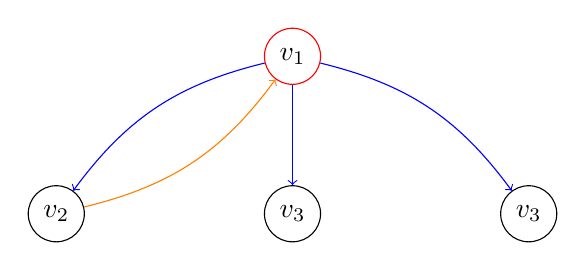
\begin{tikzpicture} 
                \node[shape=circle,draw=red] (A) at (0,0) {$v_1$};
                \node[shape=circle,draw=black] (B) at (-3,-2) {$v_2$};
                \node[shape=circle,draw=black] (C) at (0,-2) {$v_3$};
                \node[shape=circle,draw=black] (D) at (3,-2) {$v_3$};


                \path [->, draw=blue] (A) edge [bend right=20] node[right] {} (B);
                \path [->, draw=orange] (B) edge [bend right=20] node[right] {} (A);
                \path [->, draw=blue] (A) edge node[right] {} (C);
                \path [->, draw=blue] (A) edge [bend left=20] node[right] {} (D);
            \end{tikzpicture}
            \caption{esempio con ${In\text{-}deg(v_1) = 1}$ e ${Out\text{-}deg(v_1) = 3}$ } 
            \label{fig:in_out}
    \end{figure}
	\QEDA
\end{ese}

\begin{thm}
In ogni grafo orientato semplice $G=(V,A)$ sono uguali tra loro: la somma dei gradi
uscenti dei nodi, la somma dei gradi entranti dei nodi, il numero di archi del grafo.
\begin{equation}
{\sum_{v \in V}^{} In\text{-}deg(v)} = {\sum_{v \in V}^{} Out\text{-}deg(v)} = |A|
\label{eq:thm2}
\end{equation}
\proof
    Per induzione su $m = |A|$:\\
    \emph{caso base: $m = 0$}\\ 
    \indent $\sum_{v \in V}^{} In\text{-}deg(v) = \sum_{v \in V}^{} Out\text{-}deg(v) =
    m = |A| = 0$.\\
    \emph{passo induttivo:} $P(m-1) \implies P(m)$\\
    \indent sia $G=(V,E)$ un grafo orientato con $m$ archi. Si suppone che~\ref{eq:thm2} 
    sia valida $\forall$~grafo orientato con $m-1$ archi.\\
    Sia $(\bar{u}, \bar{v}) \in A$ e sia 
    $G'=(V, \text{ } A'=A \setminus \{\text{ } (\bar{u}, \bar{v}) \text{ }\})$ 
    ottenuto da $G$ togliendo $(\bar{u}, \bar{v})$. Allora:\footnote{
        Si somma $1$ perché in $G$ ci sono un arco entrante in più su $\bar{v}$ ed uno
        uscente in più da $\bar{u}$ dato che $(\bar{u},\bar{v}) \in A$.}
    \begin{align*}
        \sum_{v \in V}^{} {In\text{-}deg_{G}(v)} & = \sum_{v \in V}^{} {In\text{-}deg_{G'}(v)} + 1\\
        \sum_{v \in V}^{} Out\text{-}deg_{G}(v) & = \sum_{v \in V}^{} Out\text{-}deg_{G'}(v) + 1
    \end{align*}
    $|A'| = |A| - 1 = m - 1$ e
    \begin{align*}
        \sum_{v \in V}^{} {In\text{-}deg_{G'}(v)} & = \sum_{v \in V}^{} {Out\text{-}deg_{G'}(v)} = 
        m - 1 = |A'|
    \end{align*}
    Quindi in $G'$ vale l'ipotesi induttiva.\\Ora in $G$:
    \begin{equation*}
    \begin{split}
        |A| & = \sum_{v \in V}^{} {In\text{-}deg_{G}(v)} = \sum_{v \in V}^{} {Out\text{-}deg_{G}(v)}\\
    & =\underbrace{\underbrace{\sum_{v \in V}^{} {In\text{-}deg_{G'}(v)}}_{|A'| = m-1}+1}_{m=|A|} =
        \underbrace{\underbrace{\sum_{v \in V}^{} {Out\text{-}deg_{G'}(v)}}_{|A'| = m-1}+1}_{m=|A|}
    \end{split}
    \end{equation*}
\endproof
\end{thm}

\section{Sottografi}
\begin{defn}[sottografo]
Dato  $G=(V,E)$ grafo non orientato semplice, un suo \emph{sottografo} è un grafo
$G'=(V',E')$ con $V' \subseteq V$ e $E' \subseteq E$.
\end{defn}

\begin{defn}[sottografo indotto]
Dato  $G=(V,E)$ grafo non orientato semplice, un suo \emph{sottografo indotto} è un 
suo sottografo ${G'=(V',E')}$ tale che ${\forall (u,v) \in E}$, se
${u,v \in V' \implies (u,v) \in E'}$.
\end{defn}

\begin{ese}
In Figura~\ref{fig:sottografi} sono rappresentati un grafo ${G=(V,E)}$, un suo sottografo
$G'=(V' = \{a,d,f,e\}, E'= \{ (a,d), (a,f) \})$ ed un suo sottografo indotto (da~$V'$)
$G''=(V', E''= \{ (a,d), (a,f), (d,f), (f,e) \})$.
\begin{figure}[H]
    \centering
    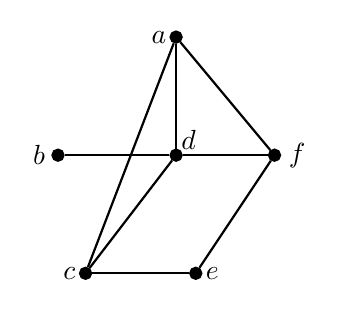
\begin{tikzpicture}[thick,scale=0.5]
        \begin{scope}[every node/.style={circle,thick,draw,fill=black,
                        inner sep=0pt, minimum size=4pt}]
            \node (A) at (0,0) [label=left:$a$]{};
            \node (B) at (0,-3) [label=60:$d$]{};
            \node (C) at (-3,-3) [label=left:$b$]{};
            \node (D) at (2.5,-3) [label=right:$f$]{};
            \node (E) at (-2.3,-6) [label=left:$c$]{};
            \node (F) at (0.5,-6) [label=right:$e$]{};
        \end{scope}

        \path (A) edge node {} (B);
        \path (A) edge node {} (D);
        \path (A) edge node {} (E);
        \path (B) edge node {} (C);
        \path (B) edge node {} (D);
        \path (B) edge node {} (E);
        \path (D) edge node {} (F);
        \path (E) edge node {} (F);
    \end{tikzpicture}
    \hspace{1cm}
    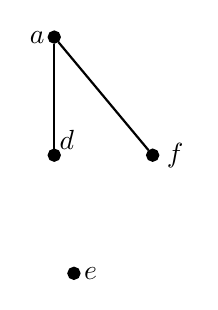
\begin{tikzpicture}[thick,scale=0.5]
        \begin{scope}[every node/.style={circle,thick,draw,fill=black,
                        inner sep=0pt, minimum size=4pt}]
        \node (A) at (0,0) [label=left:$a$]{};
        \node (B) at (0,-3) [label=60:$d$]{};
        \node (C) at (2.5,-3) [label=right:$f$]{};
        \node (D) at (0.5,-6) [label=right:$e$]{};
        \end{scope}
        \path (A) edge node {} (B);
        \path (A) edge node {} (C);
    \end{tikzpicture}
    \hspace{1cm}
    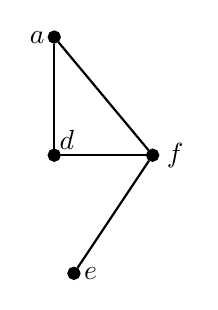
\begin{tikzpicture}[thick,scale=0.5]
        \begin{scope}[every node/.style={circle,thick,draw,fill=black,
                        inner sep=0pt, minimum size=4pt}]
            \node (A) at (0,0) [label=left:$a$]{};
            \node (B) at (0,-3) [label=60:$d$]{};
            \node (C) at (2.5,-3) [label=right:$f$]{};
            \node (D) at (0.5,-6) [label=right:$e$]{};
        \end{scope}
        \path (A) edge node {} (B);
        \path (A) edge node {} (C);
        \path (B) edge node {} (C);
        \path (C) edge node {} (D);
    \end{tikzpicture}
    \caption{Rispettivamente: un grafo $G=(V,E)$, un suo sottografo ed un suo sottografo indotto.}
    \label{fig:sottografi}
    \end{figure}
	\QEDA
\end{ese}

\section{Grafi bipartiti}
Riprendiamo ora la discussione sui grafi bipartiti che sono stati definiti a pagina~\pageref{bip}.
Un grafo è \emph{bipartito} se i suoi vertici sono partizionati in due sottoinsiemi,
$V_1$ e $V_2$ ed ogni spigolo è incidente in un vertice di $V_1$ e uno di $V_2$.
Il minimo numero di spigoli che un grafo bipartito può avere è $0$, mentre il massimo é 
$|V_1|\cdot|V_2|$.

\begin{prop}[condizione necessaria e sufficiente per grafi bipartiti]
Se $G=(V,E)$ è un grafo bipartito e $G'=(V',E')$ è un suo sottografo allora
$G'=(V',E')$ è bipartito.
Questo equivale a dire che $G'$ non è bipartito~$\iff \text{ } G$~non è bipartito. 
\end{prop}

\begin{thm}
Un grafo~$G=(V,E)$ è bipartito~$\iff$~ogni circuito di $G$ ha lunghezza pari
(la lunghezza di un circuito è il numero degli spigoli).
\end{thm}
%\begin{comment}
\proof
Consideriamo solamente i grafi connessi dato che ogni circuito è contenuto in una componente
connessa e se le componenti connesse sono bipartite allora anche il grafo è bipartito.\\
$\Longrightarrow)$ Sia $G$ un grafo bipartito e ${c = x_1\text{ - }\dots\text{ - }x_k\text{ - }x_1}$
un suo circuito di lunghezza $k$ (in Figura~\ref{fig:circuito_dim}).
Per la definizione di grafo bipartito i nodi del circuito devono essere del tipo:
${x_1 \in V_1,}\text{ }{x_2 \in V_2,}\text{ }{x_3 \in V_1,\text{ }\dots}$\\ 
Più precisamente: ${x_j \in V_1}$ se~$j$ è dispari e ${x_j \in V_2}$ se~$j$ è pari, con
${j = 1,\dots,k}$.\\
Poiché ${(x_1, x_k) \in E} \text{, } {x_1 \in V_1 \implies x_k \in V_2 \implies k}$ è pari
e, per come è stato definito il circuito, questo ha lunghezza $k$.\\
$\Longleftarrow)$ Sia $G$ un grafo con tutti i circuiti di lunghezza pari. Sia $v \in V$,
lo ''mettiamo'' in $V_1$, tutti i suoi adiacenti li ''mettiamo'' in $V_2$, poi prendiamo
tutti i vertici distanti 2 da $v$ e li mettiamo in $V_1$ \dots e così via.
In generale se esiste un cammino di lunghezza pari che parte da $v$ ed arriva fino ad un certo
nodo $n$, allora mettiamo $n$ in $V_1$, se invece il cammino ha lunghezza dispari allora
mettiamo $n$ in $V_2$.
Non possono esistere spigoli che collegano due nodi che si trovano entrambi in $V_1$ o in $V_2$.
Supponiamo che $\exists u,w$ tali che entrambi appartengono a $V_1$, che ${\exists (u,w) \in E}$;
deve esistere un cammino ${c = u - \dots - z - w}$ di lunghezza pari (quindi con ${z \in V_2}$),
se alla fine del cammino si aggiunge lo spigolo~$(u,w)$ allora si ottiene un circuito formato da
due cammini, il primo è~$c$ che ha lungheza pari ed il secondo è $(u,v)$ che ha lunghezza dispari.
Il circuito allora ha lunghezza dispari, ma è assurdo perchè la nostra ipotesi assume che $G$ 
sia un grafo che ha solo circuiti di lunghezza pari. Un ragionamento analogo lo si può fare se
$u$ e $w$ appartengono a $V_2$.
\begin{figure}[H]
    \centering
    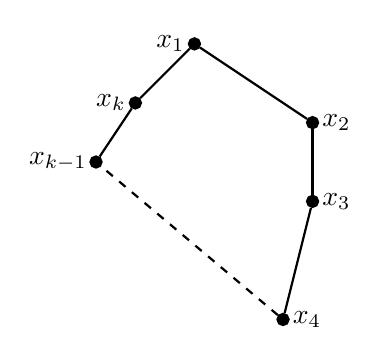
\begin{tikzpicture}[thick,scale=0.5]
        \begin{scope}[every node/.style={circle,thick,draw,fill=black,
                        inner sep=0pt, minimum size=4pt}]
            \node (A) at (0,0) [label=left:$x_1$]{};
            \node (B) at (3,-2) [label=right:$x_2$]{};
            \node (C) at (3,-4) [label=right:$x_3$]{};
            \node (D) at (2.25,-7) [label=right:$x_4$]{};
            \node (E) at (-2.5,-3) [label=left:$x_{k-1}$]{};
            \node (F) at (-1.5,-1.5) [label=left:$x_k$]{};
        \end{scope}

        \path (A) edge node {} (B);
        \path (B) edge node {} (C);
        \path (C) edge node {} (D);
        \path (D) edge node {} (E) [dashed];
        \path (E) edge node {} (F);
        \path (F) edge node {} (A);
    \end{tikzpicture}
    \caption{circuito parte $\Longrightarrow)$ della dimostrazione}
    \label{fig:circuito_dim}
\end{figure}
\endproof


\begin{algorithm}
\caption{Algoritmo per verifica bipartizione di un grafo}\label{alg:algo_bipartizione}
\begin{algorithmic} 
\STATE Da ripetere $\forall$ componente connessa di $G=(V,E)$:
\STATE $V_1 = V_2 = \emptyset$
\STATE prendo un qualsiasi $v \in V$ e lo metto in $V_1$
\FORALL{$u \in V_1 \cup V_2$}
    \STATE\COMMENT{La prima volta entro per forza nell'if perché $u$ può essere solo uguale a $v$}
    \IF{$u \in V_1$}
        \STATE aggiungo a $V_2$ tutti i vertici adiacenti a $u$ che non sono in $V_1 \cup V_2$
    \ELSE
        \STATE aggiungo a $V_1$ tutti i vertici adiacenti a $u$ che non sono in $V_1 \cup V_2$
    \ENDIF
\ENDFOR
\STATE $G$ è bipartito $\iff$ ogni spigolo ha una estremità in $V_1$ ed una in $V_2$

\end{algorithmic}
\end{algorithm}

\section{Connettività e tagli}
\begin{defn}[Connessione di 2 vertici] Sia $G=(V,E)$ un grafo non orientato 
	e siano $u,v \in V$. $u$ e $v$ sono \emph{connessi} se esiste 
	un cammino che ha come estremità $u$ e $v$.
\end{defn}
\noindent La connessione è una relazione di equivalenza nell'insieme $V$ dei vertici:
\begin{itemize}
	\item{$u$ è connesso a se stesso (riflessività)}
	\item{$u$ è connesso a $v \implies v$ è connesso a $u$ (simmetria)}
	\item{$u$ è connesso a $v$ e $v$ è connesso a $t \implies u$ è connesso a $t$ (transitività)}
\end{itemize}
$u$ e $v$ sono connessi solo se, partizionato $V$ in $V_1, V_2, \dots, V_k$ insiemi, sia $u$
che $v$ appartengono allo stesso insieme $V_i$ (con $1 \leqslant i \leqslant k$).
I $k$ insiemi rappresentano le \emph{componenti connesse} del grafo $G$. Tale grafo
$G$ è \emph{connesso} se esiste una unica partizione\footnote{Una \emph{partizione} di~$V$ è una
	sua scomposizione in parti disgiunte} (quindi $k = 1$), altrimenti si dice
\emph{sconnesso} ($k \geqslant 1$). Le componenti connesse di un grafo sono i suoi sottografi
connessi massimali.

\begin{ese} In Figura~\ref{fig:connesso_sconnesso} sono rappresentati un grafo connesso
	ed un grafo sconnesso con 3 componenti connesse.
	\begin{figure}[H]
		\centering
		\begin{subfigure}[grafo connesso]{{0.31\textwidth}}
			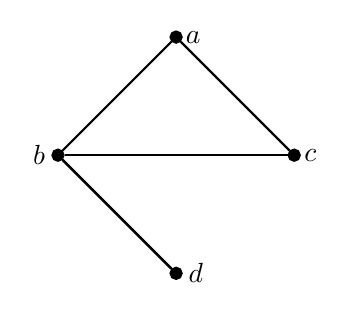
\begin{tikzpicture}[thick,scale=0.5]
			\begin{scope}[every node/.style={circle,thick,draw,fill=black,
				inner sep=0pt, minimum size=4pt}]
			\node (A) at (0,0) [label=right:$a$]{};
			\node (B) at (-3,-3) [label=180:$b$]{};
			\node (C) at (3,-3) [label=right:$c$]{};
			\node (D) at (0,-6) [label=right:$d$]{};
			\end{scope}
			
			\path (A) edge node {} (B);
			\path (A) edge node {} (C);
			\path (B) edge node {} (C);
			\path (B) edge node {} (D);
			\path (D) edge node {} (B);
			\end{tikzpicture}
			\caption{grafo connesso} 
			\label{fig:connessione}
		\end{subfigure}
		\hspace*{1cm}%\hspace*{\fill}
		\begin{subfigure}[grafo sconnesso]{{0.31\textwidth}}
			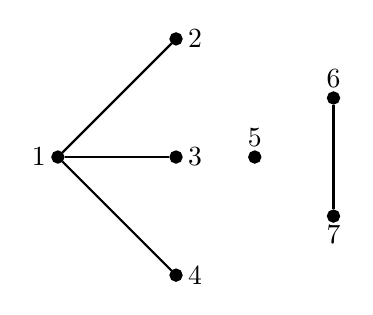
\begin{tikzpicture}[thick,scale=0.5]
			\begin{scope}[every node/.style={circle,thick,draw,fill=black,
				inner sep=0pt, minimum size=4pt}]
			\node (A) at (0,0) [label=left:$1$]{};
			\node (B) at (3,3) [label=right:$2$]{};
			\node (C) at (3,0) [label=right:$3$]{};
			\node (D) at (3,-3) [label=right:$4$]{};
			\node (E) at (5,0) [label=90:$5$]{};
			\node (F) at (7,1.5) [label=90:$6$]{};
			\node (G) at (7,-1.5) [label=270:$7$]{};
			\end{scope}
			
			\path (A) edge node {} (B);
			\path (A) edge node {} (C);
			\path (A) edge node {} (D);
			\path (F) edge node {} (G);
			\end{tikzpicture}
			\caption{grafo sconnesso con 3 componenti connesse} 
			\label{fig:sconnesso}
		\end{subfigure}
		\caption{un grafo connesso ed un grafo sconnesso} 
		\label{fig:connesso_sconnesso}
	\end{figure}
	\QEDA
\end{ese}

\begin{ese} In Figura~\ref{fig:com_conn_grafo} sono rappresentati un grafo e le sue componenti
	connesse (ovvero i suoi sottografi connessi massimali).
	\begin{figure}[H]
		\centering
		\begin{subfigure}{{0.31\textwidth}}
			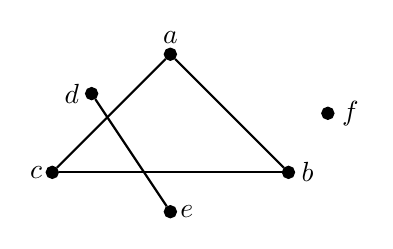
\begin{tikzpicture}[thick,scale=0.5]
			\begin{scope}[every node/.style={circle,thick,draw,fill=black,
				inner sep=0pt, minimum size=4pt}]
			\node (A) at (0,0) [label=90:$a$]{};
			\node (B) at (3,-3) [label=right:$b$]{};
			\node (C) at (-3,-3) [label=left:$c$]{};
			\node (D) at (-2,-1) [label=left:$d$]{};
			\node (E) at (0,-4) [label=right:$e$]{};
			\node (F) at (4,-1.5) [label=right:$f$]{};
			\end{scope}
			
			\path (A) edge node {} (B);
			\path (A) edge node {} (C);
			\path (B) edge node {} (C);
			\path (D) edge node {} (E);
			\end{tikzpicture}
			\caption{un grafo $G$} 
			\label{fig:connessione}
		\end{subfigure}
		\hspace*{1cm}%\hspace*{\fill}
		\begin{subfigure}{0.31\textwidth}
			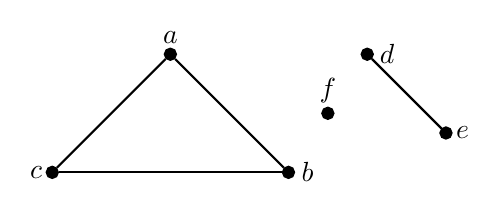
\begin{tikzpicture}[thick,scale=0.5]
			\begin{scope}[every node/.style={circle,thick,draw,fill=black,
				inner sep=0pt, minimum size=4pt}]
			\node (A) at (0,0) [label=90:$a$]{};
			\node (B) at (3,-3) [label=right:$b$]{};
			\node (C) at (-3,-3) [label=left:$c$]{};
			\node (D) at (5,0) [label=right:$d$]{};
			\node (E) at (7,-2) [label=right:$e$]{};
			\node (F) at (4,-1.5) [label=90:$f$]{};
			\end{scope}
			
			\path (A) edge node {} (B);
			\path (A) edge node {} (C);
			\path (B) edge node {} (C);
			\path (D) edge node {} (E);
			\end{tikzpicture}
			\caption{le componenti connesse di $G$} 
			\label{fig:comp_conn}
		\end{subfigure}
		\caption{un grafo e le sue componenti connesse} 
		\label{fig:com_conn_grafo}
	\end{figure}
	\QEDA
\end{ese}

\begin{defn}[taglio]
	Sia ${G=(V,E)}$ un grafo non orientato e sia ${S \subseteq V}$. Il \emph{taglio} (\emph{cut})
	associato ad~$S$ è l'insieme degli \emph{spigoli che hanno esattamente una estremità} 
	in~$S$ e si indica con~$\delta(S)$.
	\[ \delta(S) = \{(u,v) \in E \colon | S \cap \{u,v\} | = 1 \} \]
\end{defn}
Si dice che $\delta(S)$ separa $u$ e $v$ se ${|S \cap \{u,v\}| = 1}$.

\begin{ese}
	esempio: ${V=\{a,b,c,d,e\}}$ sono i nodi del grafo in Figura~\ref{fig:es_taglio} che, ha come
	taglio associato ad ${S = \{a, b\}}$ l'insieme ${\delta(S)= \{(a,d),(a,c),(b,c),(b,e)\}}$.
	\begin{figure}[H]
		\centering
		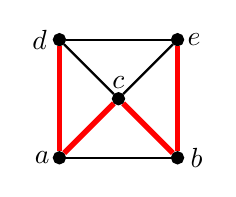
\begin{tikzpicture}[thick,scale=0.5]
		\begin{scope}[every node/.style={circle,thick,draw,fill=black,
			inner sep=0pt, minimum size=4pt}]
		\node (A) at (0,0) [label=left:$a$]{};
		\node (B) at (3,0) [label=right:$b$]{};
		\node (C) at (1.5,1.5) [label=90:$c$]{};
		\node (D) at (0,3) [label=left:$d$]{};
		\node (E) at (3,3) [label=right:$e$]{};
		\end{scope}
		
		\path (A) edge node {} (B);
		\path [draw=red,line width=0.2em](A) edge node {} (C);
		\path [draw=red,line width=0.2em](B) edge node {} (C);
		\path (D) edge node {} (E);
		\path [draw=red,line width=0.2em](A) edge node {} (D);
		\path [draw=red,line width=0.2em](B) edge node {} (E);
		\path (C) edge node {} (D);
		\path (C) edge node {} (E);
		\path (D) edge node {} (E);
		\end{tikzpicture}
		\caption{Taglio associato ad $S = \{ a, b \}$} 
		\label{fig:es_taglio}
	\end{figure}
	\QEDA
\end{ese}

\begin{thm}
	Sia ${P = u - \dots - v}$ un cammino su un grafo ${G=(V,E)}$ e sia $\delta(S)$ un taglio che
	separa $u$ da~$v$, allora ${ |P \cap \delta(S)| \geqslant 1 }$. \footnote{Con
		${P \cap \delta(S)}$ facciamo riferimento all'intersezione dell'insieme formato da
		tutti gli spigoli che sono parte del cammino $P$ con $\delta(S)$}
	\label{thm:taglio_cammino}
\end{thm}
\proof
%Poichè esiste un cammino $P$ tra $u$~e~$v$ questo vuol dire che i due nodi sono connessi.
Per la definizione di taglio ${\exists S \subset V}$ in cui ${u \in S}$ o ${v \in S}$ ma,
sia $u$ che $v$ non possono appertenere entrambi allo stesso insieme $S$. Supponiamo che
${u \in S}$ (un ragionamento analogo lo si può fare per $v$), allora 
\textcolor{red}{DA TERMINARE!!! Lemma 1.3.1 pag 14 Conforti-Faenza}
\endproof

\begin{thm}
	Sia $G=(V,E)$ un grafo non orientato, allora ${u,v \in V}$ appartengono alla stessa 
	componente connessa di ${G \iff \delta(S) \neq \emptyset \text{ } \forall 
		\delta(S\neq \emptyset)}$ che separa $u$ e~$v$.
\end{thm}
\proof
Sia ${G=(V,E)}$ un grafo non orientato connesso, sia ${S \subseteq V}$, ${S \neq \emptyset}$ e
sia $\delta(S)$ un taglio di~$G$ che separa due nodi $u$ e~$v$. Dato che $G$ è connesso allora
esiste un cammino $P$ tra $u$ e~$v$, per il Teorema~\ref{thm:taglio_cammino} sappiamo che
${ |P \cap \delta(S)| \geqslant 1 }$ quindi ${\delta(S) \neq \emptyset}$.
\textcolor{red}{DA TERMINARE!!! Lemma 1.3.3 pag 14 Conforti-Faenza}
\endproof

%\begin{algorithm}
%	\caption{Algoritmo che determina se $\exists$ un cammino tra $u$~e~$v$ }\label{alg:algo_bipartizione}
%	\begin{algorithmic}
%		\REQUIRE{un grafo ${G=(V,E)}$ ed un suo vertice ${v \in V}$}
%		\ENSURE{Una comp. connessa $C$ che contiene~$v$ (tutti i nodi raggiungibili da $v$)}
%		\STATE $C = \emptyset$
%		\STATE prendo $v$ e lo metto in $C$ \COMMENT{proprietà riflessiva: $v$ è connesso a se stesso}
%		\STATE \COMMENT{Adesso esamino tutti i nodi che sono nella comp. connessa.}
%		\FORALL{$u \in C$}
%		\STATE aggiungo a $C$ tutti i vertici adiacenti a $u$ che non sono già in $C$
%		\ENDFOR
%		\STATE \COMMENT{ora $C$ è la componente connessa che contieve $v$, se contiene 
%			anche $u$ allora $\exists$~un cammino tra $u$ e~$v$}
%		
%	\end{algorithmic}
%\end{algorithm}
\begin{codebox}
	\Procname{$\proc{Cammino-Minimo}(G, v)$}
	\li \Comment{${G=(V,E)}$ è un grafo e ${v \in V}$ è un suo vertice}
	\li \Comment{l'lgoritmo determina se $\exists$ un cammino tra i vertici $u$~e~$v$ }
	\li \id{C} $\gets \emptyset$
	\li \id{C} $\leftarrow v$ \Comment{prendere $v$ e metterlo nell'insieme $C$ }
	\li \Comment{Si esaminano tutti i nodi nella componente connessa}
	\li \For each ${v \in V}$
	\li \Do
	Aggiungere a $C$ tutti i vertici adiacenti ad $u$ che non sono già in $C$
	\End
	\li \Comment{Arrivati a questo punto, $C$ è la componente connessa che contieve $v$}
	\li \Comment{se contiene anche $u$ allora $\exists$~un cammino tra $u$ e~$v$}
	\li \Comment{notare che $\delta(C) \neq \emptyset$}
\end{codebox}

\begin{defn}[connettività sugli spigoli]
	Sia ${G=(V,E)}$ un grafo connesso. Si dice connettività
	sugli spigoli e si indica con~$\lambda(G)$ il minimo numero di spigoli la cui rimozione 
	trasforma $G$ in un grafo sconnesso.
\end{defn}

\section{Grafi isomorfi}
\begin{defn}[grafi isomorfi]
Due grafi $G=(V,E)$ e $G'=(V',E')$ sono \emph{isomorfi} se esiste una corrispondenza biunivoca
(\emph{isomorfismo}) tra i vertici di $V$ e quelli di $V'$ tale che: due vertici di $V$ sono
adiacenti in $G \iff $ i corrispondenti vertici di $V'$ sono adiacenti in $G'$. 
\end{defn}
Stabilire se due grafi sono isomorfi è un problema difficile, per 
sapere se lo sono si può ''cercare l'isomorfismo''.
Due grafi sono isomorfi se:\footnote{sono condizioni necessarie ma \emph{non sufficienti}}
\begin{enumerate}
    \item hanno lo stesso numero di vertici
    \item hanno lo stesso numero di spigoli
    \item hanno lo stesso numero di vertici con lo stesso grado
    \item hanno gli stessi sottografi indotti
    \item i loro complementari devono essere isomorfi
\end{enumerate}

\begin{ese}
In Figura~\ref{fig:isomorfi} sono rappresentati 2 grafi isomorfi
\begin{figure}[H]
    \centering
    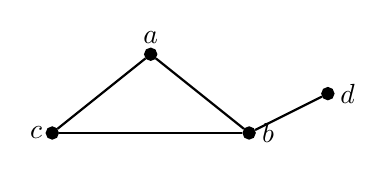
\begin{tikzpicture}[thick,scale=0.5]
        \begin{scope}[every node/.style={circle,thick,draw,fill=black,
                        inner sep=0pt, minimum size=4pt}]
            \node (A) at (0,0) [label=90:$a$]{};
            \node (B) at (-2.5,-2) [label=left:$c$]{};
            \node (C) at (2.5,-2) [label=right:$b$]{};
            \node (D) at (4.5,-1) [label=right:$d$]{};
        \end{scope}

        \path (A) edge node {} (B);
        \path (B) edge node {} (C);
        \path (C) edge node {} (A);
        \path (C) edge node {} (D);
    \end{tikzpicture}
    \hspace{1cm}
    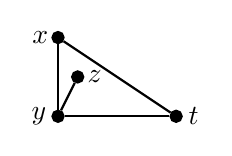
\begin{tikzpicture}[thick,scale=0.5]
        \begin{scope}[every node/.style={circle,thick,draw,fill=black,
                        inner sep=0pt, minimum size=4pt}]
            \node (A) at (0,0) [label=left:$x$]{};
            \node (B) at (0,-2) [label=left:$y$]{};
            \node (C) at (0.5,-1) [label=right:$z$]{};
            \node (D) at (3,-2) [label=right:$t$]{};
        \end{scope}

        \path (A) edge node {} (B);
        \path (B) edge node {} (C);
        \path (B) edge node {} (D);
        \path (D) edge node {} (A);
    \end{tikzpicture}
    \hspace{1cm}
    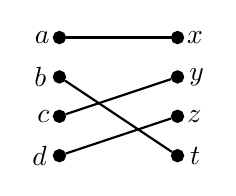
\begin{tikzpicture}[thick,scale=0.5]
        \begin{scope}[every node/.style={circle,thick,draw,fill=black,
                        inner sep=0pt, minimum size=4pt}]
            \node (A) at (0,0) [label=left:$a$]{};
            \node (B) at (3,0) [label=right:$x$]{};
            \node (C) at (0,-1) [label=left:$b$]{};
            \node (D) at (3,-1) [label=right:$y$]{};
            \node (E) at (0,-2) [label=left:$c$]{};
            \node (F) at (3,-2) [label=right:$z$]{};
            \node (G) at (0,-3) [label=left:$d$]{};
            \node (H) at (3,-3) [label=right:$t$]{};
        \end{scope}

        \path (A) edge node {} (B);
        \path (C) edge node {} (H);
        \path (E) edge node {} (D);
        \path (G) edge node {} (F);
    \end{tikzpicture}
    \caption{2 grafi isomorfi} \label{fig:isomorfi}
\end{figure}
\QEDA
\end{ese}

\begin{ese}
In Figura~\ref{fig:compl_iso} sono rappresentati 2 grafi complementari non isomorfi
\begin{figure}[H]
    \centering
    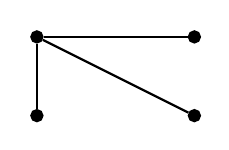
\begin{tikzpicture}[thick,scale=0.5]
        \begin{scope}[every node/.style={circle,thick,draw,fill=black,
                        inner sep=0pt, minimum size=4pt}]
            \node (A) at (0,0) {};
            \node (B) at (0,-2) {};
            \node (C) at (4,0) {};
            \node (D) at (4,-2) {};
        \end{scope}

        \path (A) edge node {} (B);
        \path (A) edge node {} (C);
        \path (A) edge node {} (D);
    \end{tikzpicture}
    \hspace{1cm}
    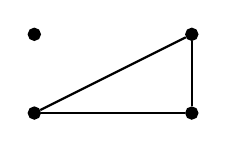
\begin{tikzpicture}[thick,scale=0.5]
        \begin{scope}[every node/.style={circle,thick,draw,fill=black,
                        inner sep=0pt, minimum size=4pt}]
            \node (A) at (0,0) {};%[label=left:$a$]{};
            \node (B) at (0,-2) {};%[label=left:$b$]{};
            \node (C) at (4,0) {};%[label=right:$c$]{};
            \node (D) at (4,-2) {};%[label=right:$d$]{};
        \end{scope}

        \path (B) edge node {} (C);
        \path (B) edge node {} (D);
        \path (C) edge node {} (D);
    \end{tikzpicture}
    \caption{2 grafi complementari non isomorfi} \label{fig:compl_iso}
\end{figure}
\QEDA
\end{ese}

Se le prime tre condizioni della lista sono verificate, si può provare a costruire il possibile 
isomorfismo controllando che la condizione 4 sia verificata. Lo si può fare costruendo sottografi
indotti \emph{accoppiando tra loro vertici che nel grafo di partenza hanno stesso grado e sono a
loro volta collegati tra loro}. 
\begin{figure}[H]
	\centering
	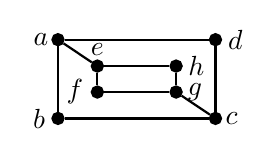
\begin{tikzpicture}[thick,scale=0.5]
	\begin{scope}[every node/.style={circle,thick,draw,fill=black,
		inner sep=0pt, minimum size=4pt}]
	\node (A) at (0,0) [label=left:$a$]{};
	\node (B) at (0,-2) [label=left:$b$]{};
	\node (C) at (4,-2) [label=right:$c$]{};
	\node (D) at (4,0) [label=right:$d$]{};
	\node (E) at (1,-0.67) [label=90:$e$]{};
	\node (F) at (1,-1.33) [label=left:$f$]{};
	\node (G) at (3,-1.33) [label=right:$g$]{};
	\node (H) at (3,-0.67) [label=right:$h$]{};
	\end{scope}
	
	\path (A) edge node {} (B);
	\path (B) edge node {} (C);
	\path (C) edge node {} (D);
	\path (D) edge node {} (A);
	\path (A) edge node {} (E);
	\path (E) edge node {} (F);
	\path (F) edge node {} (G);
	\path (G) edge node {} (H);
	\path (E) edge node {} (H);
	\path (G) edge node {} (C);
	\end{tikzpicture}
	\hspace{1cm}
	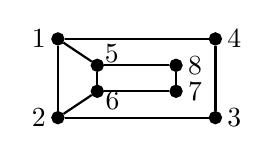
\begin{tikzpicture}[thick,scale=0.5]
	\begin{scope}[every node/.style={circle,thick,draw,fill=black,
		inner sep=0pt, minimum size=4pt}]
	\node (A) at (0,0) [label=left:$1$]{};
	\node (B) at (0,-2) [label=left:$2$]{};
	\node (C) at (4,-2) [label=right:$3$]{};
	\node (D) at (4,0) [label=right:$4$]{};
	\node (E) at (1,-0.67) [label=30:$5$]{};
	\node (F) at (1,-1.33) [label=-5:$6$]{};
	\node (G) at (3,-1.33) [label=right:$7$]{};
	\node (H) at (3,-0.67) [label=right:$8$]{};
	\end{scope}
	
	\path (A) edge node {} (B);
	\path (B) edge node {} (C);
	\path (C) edge node {} (D);
	\path (D) edge node {} (A);
	\path (A) edge node {} (E);
	\path (B) edge node {} (F);
	\path (E) edge node {} (F);
	\path (F) edge node {} (G);
	\path (G) edge node {} (H);
	\path (E) edge node {} (H);
	\end{tikzpicture}
	%\caption{} \label{fig:}
\end{figure}

\dots